\begin{enumerate}[label=\thesubsection.\arabic*.,ref=\thesubsection.\theenumi]
\numberwithin{equation}{enumi}

\item Consider an op amp having a single pole open loop response $G_{o} = 10^5$ and $f_{p} = 10$ Hz.Let op amp be ideal connected in non-inverting terminal with a nominal low frequency of closed loop gain of 100 
\subitem A manufacturing error introducing a second pole at $10^4$ Hz.Find the frequency at which $|GH| = 1$ and phase margin
\subitem What values of H phase margin is greater than 45\degree

\begin{figure}[ht!]
	\begin{center}
		\resizebox{\columnwidth/1}{!}{\tikzset{
        block/.style = {draw, rectangle,
            minimum height=1cm,
            minimum width=2cm},
        input/.style = {coordinate,node distance=1cm},
        output/.style = {coordinate,node distance=4cm},
        arrow/.style={draw, -latex,node distance=2cm},
        pinstyle/.style = {pin edge={latex-, black,node distance=2cm}},
        sum/.style = {draw, circle, node distance=1cm},
}

\begin{tikzpicture}[node distance=2.5cm,auto,>=latex']
  \node [input, name=input] {};
  \node [sum, right of=input] (sum) {};
  \node [block, right of = sum] (block1) {$G_c(s)$};
  \node [block, right of = block1] (block2) {$G(s)$};
  \node [output, right of= block2] (output) {};
  \draw [->] (input) -- node {$R(s)\ +$} (sum);
  \draw [->] (sum) -- node {} (block1);
  \draw [->] (block1) -- node {} (block2);
  \draw [->] (block2) -- node [name =y] {$Y(s)$} (output);
  \draw [->] (y) -- ++ (0,-2) -| node [pos=0.99] {$-$} (sum);
\end{tikzpicture}}
	\end{center}
	\caption{}
	\label{fig:ee18btech11034_fig}
\end{figure}

\solution Part 1 of the question
For a two-pole amplifier open loop transfer function is 

\begin{align}
    G\brak{s} = \frac{G_{o}}{\brak{1+\frac{s}{\omega_{1}}}\brak{1+\frac{s}{\omega_{2}}}}
\end{align}
Poles are at $f_{1} =10$ and $f_{2} = 10^{4}$
\begin{align}
G\brak{f} = \frac{G_{o}}{\brak{1+\j\frac{f}{f_{1}}}\brak{1+\j\frac{f}{f_{2}}}}
\\
\implies \frac{10^{5}}{\brak{1+\j\frac{f}{10}}\brak{1+\j\frac{f}{10^{4}}}}
\label{eq:ee18btech11034_1}
\end{align}
As given closed loop gain is 100
\begin{align}
    \abs T = 100
\end{align}
For nominal low frequency $|GH| \gg 1$ and from Fig.\ref{fig:ee18btech11034_fig}
\begin{align}
    T = \frac{G}{1+GH}
    \\
\implies \approx \frac{1}{H}
\end{align}
So from this 
\begin{align}
    H = 0.01
    \label{eq:ee18btech11034_2}
\end{align}
For the $|GH| = 1$ and from \eqref{eq:ee18btech11034_1} and \eqref{eq:ee18btech11034_2}
\begin{align}
   \frac{10^{3}}{\brak{\sqrt{1+\frac{f^2}{100}}}\brak{\sqrt{1+\frac{f^2}{10^{8}}}}} = 1
\end{align}
\begin{align}
    \brak{1+\frac{f^2}{100}}\brak{1+\frac{f^2}{10^{8}}} = 10^{6}
\end{align}
Solving f using python code  
\begin{align}
    f = 7861.5 
\end{align}
From definition of phase margin $\alpha = 180\degree + \phi$
where $\phi$ is the phase of GH
\begin{align}
\phi = -\tan^{-1}\brak{\frac{f}{10}} -\tan^{-1}\brak{\frac{f}{10^{4}}}
\label{eq:ee18btech11034_phaseGH}
\end{align}
At $f = 7861.5$
\begin{align}
    \phi = -128.1\degree
    \\
    \implies \alpha = 180\degree + \phi
    \label{eq:ee18btech11034_3}
    \\
    \implies \alpha = 51.9\degree
\end{align}
\textbf{Hence for frequency $f = 7861.5$ Hz $|GH| = 1$ and phase margin is 51.9\degree}

The following code for bode plot of part 1
\begin{lstlisting}
codes/ee18btech11034/ee18btech11034_1.py
\end{lstlisting}

\item Verification using Bode plot of part 1
\begin{figure}[!h]
\centering
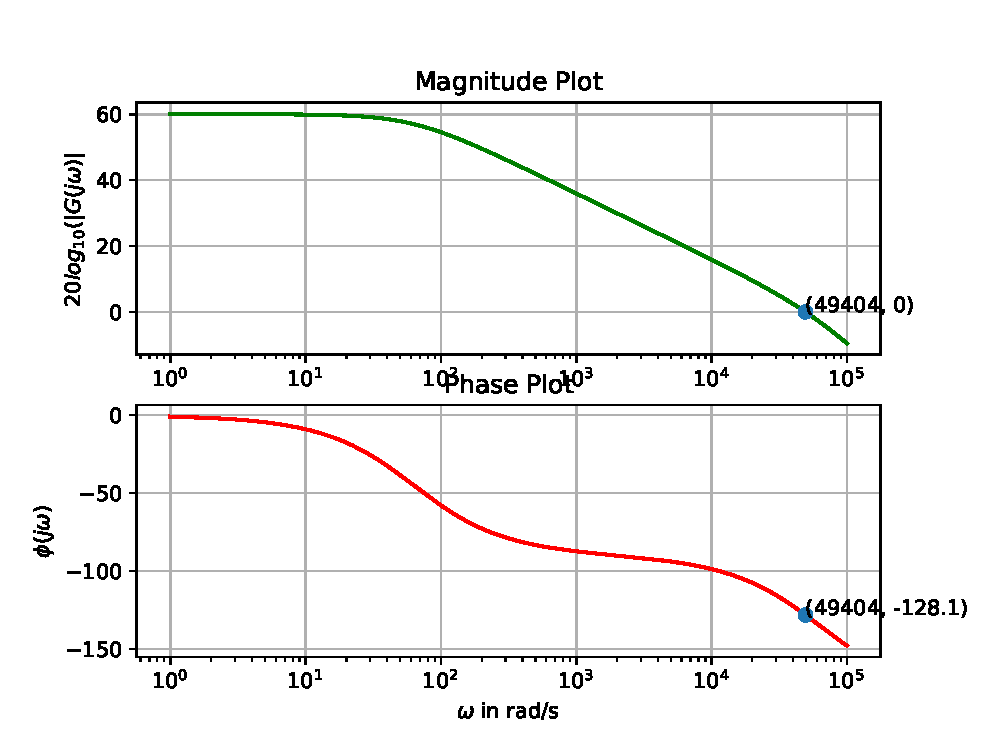
\includegraphics[width=\columnwidth]{./figs/ee18btech11034/ee18btech11034_1.eps}
\caption{}
\label{fig:ee18btech11034_1}
\end{figure}

\solution Part 2 of the question
For phase margin $\alpha=45\degree$ and from \eqref{eq:ee18btech11034_3}
\begin{align}
    \phi = -135\degree
    \label{eq:ee18btech11034_4}
\end{align}
From \eqref{eq:ee18btech11034_phaseGH} and \eqref{eq:ee18btech11034_4}
\begin{align}
    \phi = -\tan^{-1}\brak{\frac{f}{10}} -\tan^{-1}\brak{\frac{f}{10^{4}}}  = -135\degree
 \end{align}
 \begin{align}
\tan^{-1}\brak{\frac{\frac{f}{10} + \frac{f}{10^{4}}}{1-\frac{f^2}{10^{5}}}} = 135\degree
\end{align}
\begin{align}
    \frac{\frac{f}{10} + \frac{f}{10^{4}}}{1-\frac{f^2}{10^{5}}} = -1
\end{align}
Solving f using python
\begin{align}
    f \approx 10^{4}
\end{align}
For the above f equating $|GH|=1$ and from \eqref{eq:ee18btech11034_1}
\begin{align}
    \frac{\brak{10^{5}}H}{\brak{\sqrt{1+\frac{10^{8}}{100}}}\brak{\sqrt{1+\frac{10^{8}}{10^{8}}}}} = 1
\end{align}
Solving H using python code
\begin{align}
    H = 1.414 \times 10^{-2}
    \\
    \implies H_{max} =  1.414 \times 10^{-2}
\end{align}
In the part 1 of question for $H = 0.01$ which is less than $H_{max}$ phase margin is greater than 45\degree

So for 
\begin{align}
    H < H_{max} 
    \\
    \implies H < 1.414 \times 10^{-2}
\end{align}
the phase margin is greater than 45\degree

The following code for bode plot of part 2
\begin{lstlisting}
codes/ee18btech11034/ee18btech11034_2.py
\end{lstlisting}

\item Verification using Bode plot of part 2
\begin{figure}[!h]
\centering
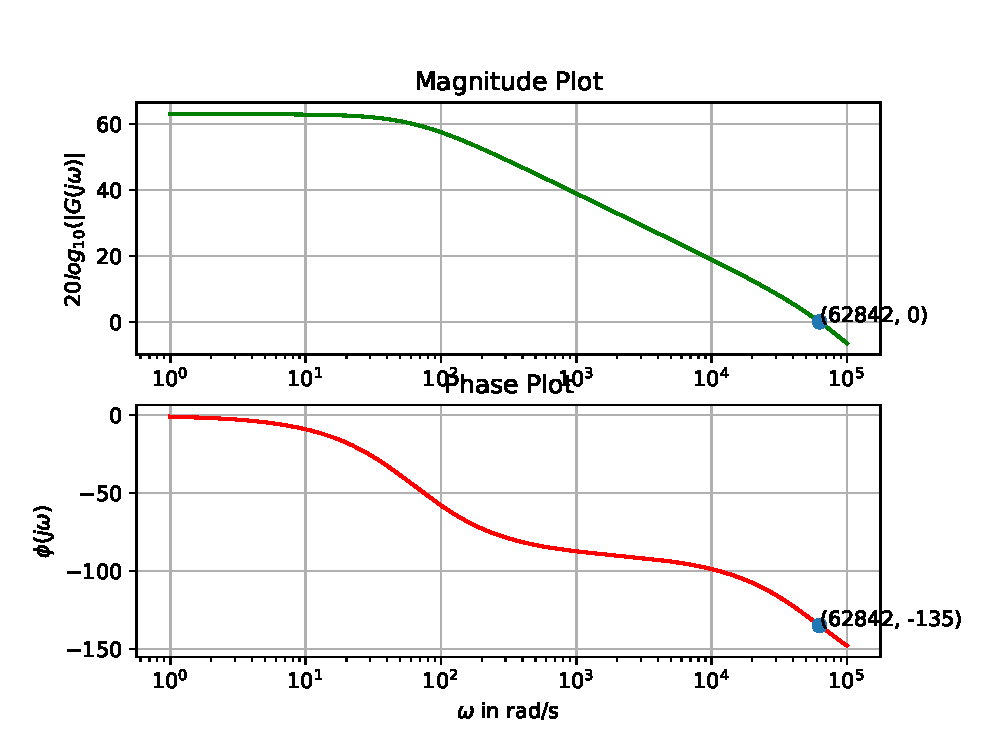
\includegraphics[width=\columnwidth]{./figs/ee18btech11034/ee18btech11034_2.eps}
\caption{}
\label{fig:ee18btech11034_2}
\end{figure}

Below is the code for computations
\begin{lstlisting}
codes/ee18btech11034/ee18btech11034.py
\end{lstlisting}

\end{enumerate}